%%%%%%%%%%%%%%%%%%%%%%%%%%%%%%%%%%%%%%%%%
% Short Sectioned Assignment
% LaTeX Template
% Version 1.0 (5/5/12)
%
% This template has been downloaded from:
% http://www.LaTeXTemplates.com
%
% Original author:
% Frits Wenneker (http://www.howtotex.com)
%
% License:
% CC BY-NC-SA 3.0 (http://creativecommons.org/licenses/by-nc-sa/3.0/)
%
%%%%%%%%%%%%%%%%%%%%%%%%%%%%%%%%%%%%%%%%%

%----------------------------------------------------------------------------------------
%	PACKAGES AND OTHER DOCUMENT CONFIGURATIONS
%----------------------------------------------------------------------------------------

\documentclass[paper=a4, fontsize=11pt]{scrartcl} % A4 paper and 11pt font size

\usepackage[T1]{fontenc} % Use 8-bit encoding that has 256 glyphs
\usepackage{fourier} % Use the Adobe Utopia font for the document - comment this line to return to the LaTeX default
\usepackage[english]{babel} % English language/hyphenation
\usepackage{amsmath,amsfonts,amsthm} % Math packages
\usepackage{multicol}
\usepackage[margin=1in]{geometry}

\usepackage{sectsty} % Allows customizing section commands
\allsectionsfont{\centering \normalfont\scshape} % Make all sections centered, the default font and small caps
% \allsectionsfont{\normalfont\scshape} % Make all sections centered, the default font and small caps

\usepackage{fancyhdr} % Custom headers and footers
\pagestyle{fancyplain} % Makes all pages in the document conform to the custom headers and footers
\fancyhead{} % No page header - if you want one, create it in the same way as the footers below
\fancyfoot[L]{} % Empty left footer
\fancyfoot[C]{} % Empty center footer
\fancyfoot[R]{\thepage} % Page numbering for right footer
\renewcommand{\headrulewidth}{0pt} % Remove header underlines
\renewcommand{\footrulewidth}{0pt} % Remove footer underlines
\setlength{\headheight}{13.6pt} % Customize the height of the header

% \numberwithin{equation}{section} % Number equations within sections (i.e. 1.1, 1.2, 2.1, 2.2 instead of 1, 2, 3, 4)
% \numberwithin{figure}{section} % Number figures within sections (i.e. 1.1, 1.2, 2.1, 2.2 instead of 1, 2, 3, 4)
% \numberwithin{table}{section} % Number tables within sections (i.e. 1.1, 1.2, 2.1, 2.2 instead of 1, 2, 3, 4)

\setlength\parindent{0pt} % Removes all indentation from paragraphs - comment this line for an assignment with lots of text

\usepackage{graphicx}

%----------------------------------------------------------------------------------------
%	TITLE SECTION
%----------------------------------------------------------------------------------------

\newcommand{\horrule}[1]{\rule{\linewidth}{#1}} % Create horizontal rule command with 1 argument of height

\title{	
    \normalfont \normalsize 
    \textsc{Fundamentals of Linear Algebra and Optimization} \\ [25pt] % Your university, school and/or department name(s)
    \horrule{0.5pt} \\[0.4cm] % Thin top horizontal rule
    \huge Project 2 \\ % The assignment title
    \horrule{2pt} \\[0.5cm] % Thick bottom horizontal rule
}

\author{Armon Shariati} % Your name

\date{\normalsize\today} % Today's date or a custom date

\begin{document}

\maketitle % Print the title

\section*{Problem 2}

Applying the \texttt{haar} function to the various strings $w$, yields a
similar waveform across the different variations, whereby the lower index
coefficients are identical and the higher index coefficients are the only ones
to change. This is consistent with the notion that the coefficient vector
produced by the haar transform captures coarse information at the lower index
coefficients and fine information at the higher index coefficients. When the
same vector is concatenated on itself multiple times, intuitively the coarser
features of the signal would remain the same, whereas the higher frequency
details may have changed.


\begin{figure}[ht] 
      \label{ fig7} 
      \begin{minipage}[b]{0.5\linewidth}
          \centering
          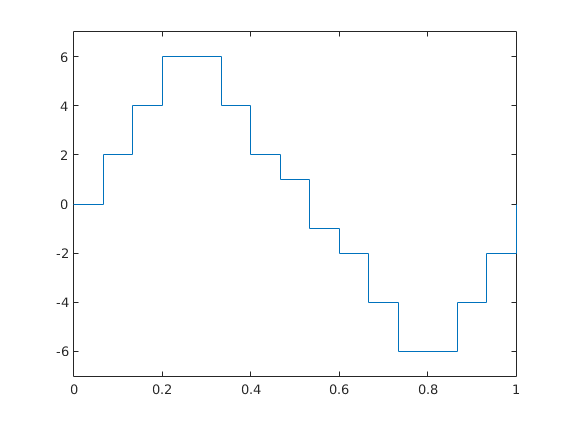
\includegraphics[width=.5\linewidth]{orig.png} 
          \caption{Original $u$.} 
          \vspace{4ex}
      \end{minipage}%%
      \begin{minipage}[b]{0.5\linewidth}
          \centering
          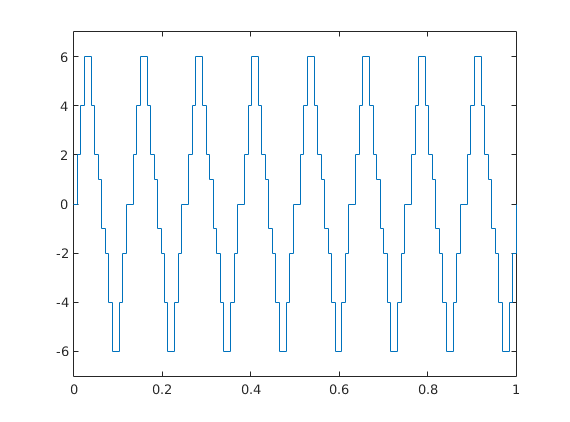
\includegraphics[width=.5\linewidth]{orig_cat.png} 
          \caption{Concatenation of $u$ with itself 8 times, $w$.} 
          \vspace{4ex}
      \end{minipage} 
      \begin{minipage}[b]{0.5\linewidth}
          \centering
          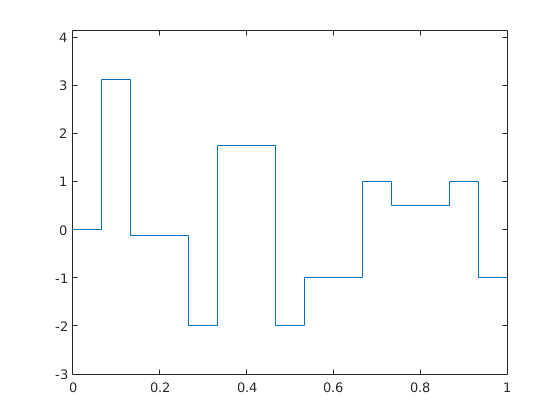
\includegraphics[width=.5\linewidth]{haar_orig.png} 
          \caption{Haar Transform of original $u$.} 
          \vspace{4ex}
      \end{minipage}%% 
      \begin{minipage}[b]{0.5\linewidth}
          \centering
          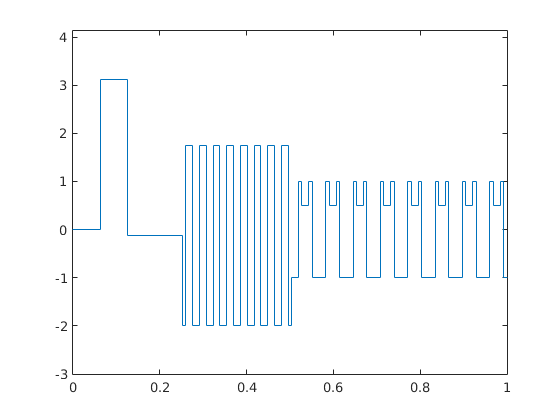
\includegraphics[width=.5\linewidth]{haar_cat.png} 
          \caption{Haar Transform of $w$.} 
          \vspace{4ex}
      \end{minipage} 
  \end{figure}

\section*{Problem 3}

Once $k=4$, zeros begin to appear in the coefficient vector $c$.  For $k=4, 5,
6, 7$, the output of the transform, $c$, no longer changes. This suggests that
despite the number of rounds of averaging and differencing, each vector has an
upper bound of compression. In other words, a point is reached where an input
vector $u$ can not be compressed further with more averaging and differencing. 

\bigskip
The result of \texttt{haar(handel, 1)} is the original song becomes duplicated and
each iteration is half as long as the original.  Furthermore, the overall
amplitude of the second iteration seems attenuated with respect to the first
iteration. When $k=2$, the same effect takes place on the first iteration of
the song from the output of $k=1$. Moreover, this yields a total of three
iterations of the song whereby the first two iterations are of the same length
and the third iteration being twice as long as both. The same attenuation
occurs to the second iteration as compared to the first iteration.  Finally,
for each $k>2$, the same thing occurs on the first instance of the song which
lives in the output of the previous $k-1$ steps. For $k=3$, there are five
iterations of the song.

\bigskip
After zeroing out the detail coefficients and reconstructing the original
signal, the song sounds much more grainy with static noise introduced to it.


\section*{Problem 4}
The third entry in the second row of the $P$ of Ames' paper, is incorrect.
This value should be $1152$ instead of $1156$.

\bigskip
After reconstructing \texttt{Xdurer} from its haar coefficients, it is
indistinguishable from the original image.


\end{document}
